\section{Dataset}
For research purposes, the GWA-T-12 BitBrain dataset\cite{shen2015statistical} is used. BitBrain dataset contains the information about performance matrices of 1750 VM which are distributed on BitBrain datacenter. BitBrain  Cloud provides services to maintain the hosting and compute the business enterprise operates on a VM, it has two dataset one with FastStorage and the second is Rnd dataset. FastStorage dataset has 1250 VM which is connected to fast storage area Network which has 1-month data with 5 min of interval. While another Rnd has 500 VM of fast storage area network and few of them are slower Network Attached Storage device, which has 3 months of data with 5 min of interval.
The following performance metrics are collected by BitBrain VM.
\begin{enumerate}
\item Timestamp: which is in Unix format from 01-01-1970.
\item CPU  capacity provisioned: which is in MHZ format.
\item CPU cores:     define the  number of cores in the CPU
\item CPU usage: which is measured in MHZ
\item CPU usage [\%]: which is percentage format
\item Disk read throughput data is in KB/s format
\item Disk write throughput:   data is in KB/s format
\item Memory usage: Memory usage measured in KB.
\item Memory capacity Provisioned:   it is in a percentage format
\item  Network transmitted throughput:  it is in KB/s format
\item  Network Received  throughput: it is in KB/s format
In this research, the Rnd dataset is more useful which has 3 months of data and more than  12 million entries of data with five minutes of interval.
\end{enumerate}

 
\section{ Data visualization and  feature engineering}
Rnd Dataset has more than 12.5 million data about performance metrics. First, convert the timestamp epoch into date format to understand the time series data. Once the timestamp is in date format then use as an index of the data frame that helps to understand the flow of performance with time. With the help of features, engineering extracts the numbers of information from timestamps like identify weekdays, weekends, months, and days of capturing data. This information is very useful to find trends or seasonality in the dataset. To run model, resample data based on hourly basis which provides a frequency of data helps to predict the model and resampling sometime discover long term pattern that is very useful when forecasting data.
After resampling data following figure 5 give data visualization based on an hourly basis of different performance matrices.




\begin{figure}[htp]

\subfloat[Transmitted throughput]{%
  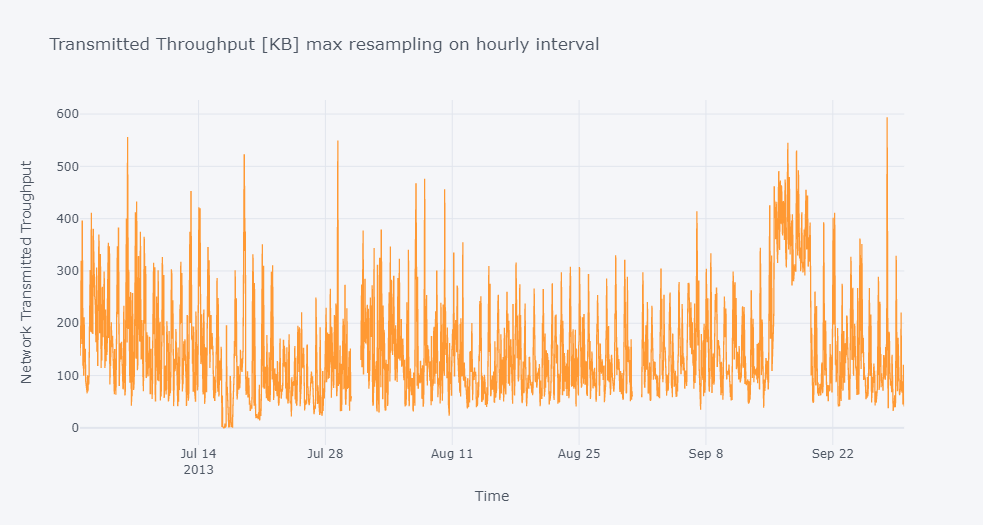
\includegraphics[width=1\linewidth,height=5cm]{DV1.png}%
}

\subfloat[Memory Usage]{
  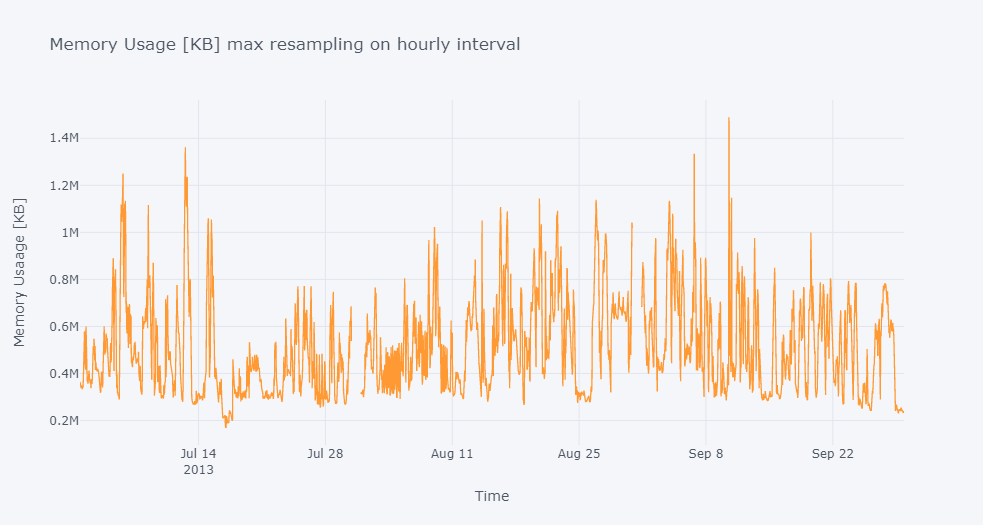
\includegraphics[width=1\linewidth,height=5cm]{DV2.png}%
}
\caption{Data Visualization of performance metrics}
\label{fig:visual1}
\end{figure}


\begin{figure}[htp]

\subfloat[CPU usage]{
  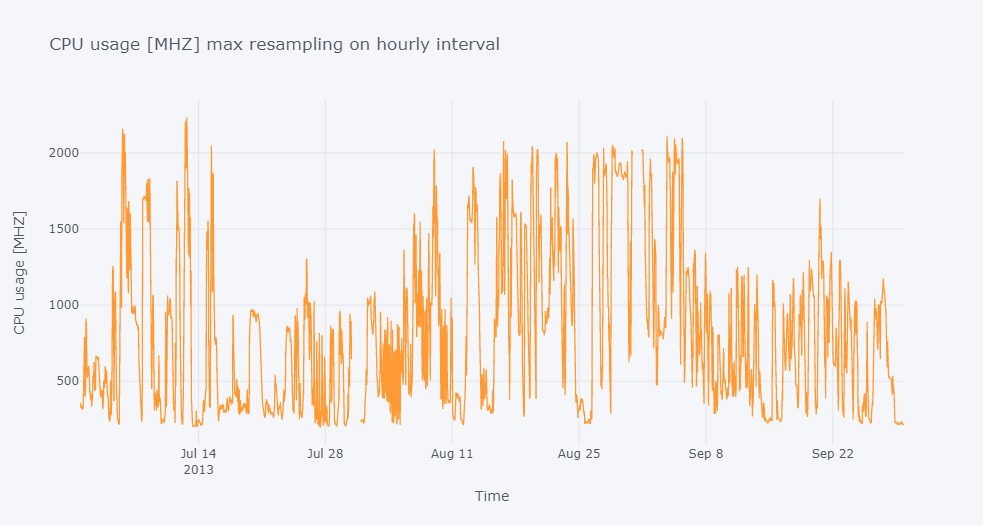
\includegraphics[width=1\linewidth,height=5cm]{DV3.png}%
}

\subfloat[Received Throughput]{
  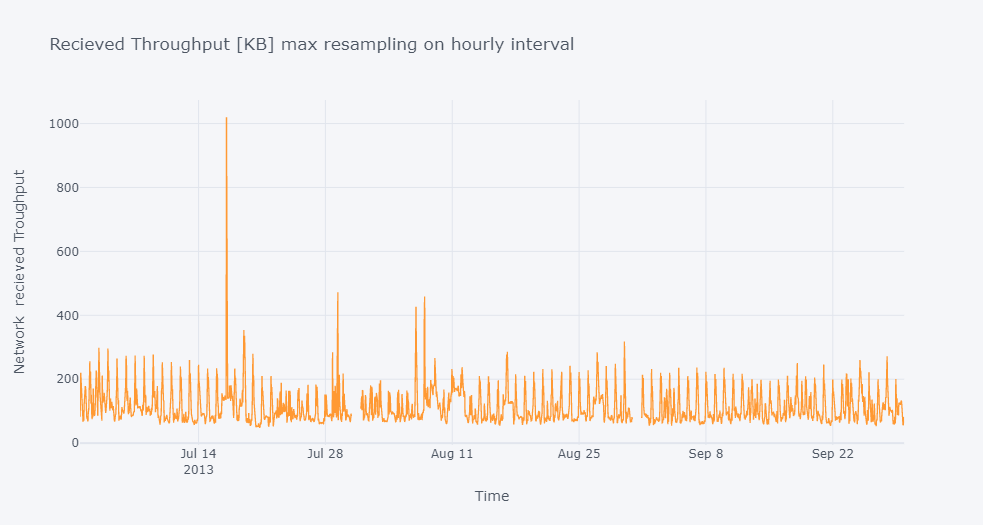
\includegraphics[width=1\linewidth,height=5cm]{DV4.png}%
}
\caption{Data Visualization of performance metrics }
\label{fig:visual}
\end{figure}



\begin{figure}[htp]

\subfloat[]{%
  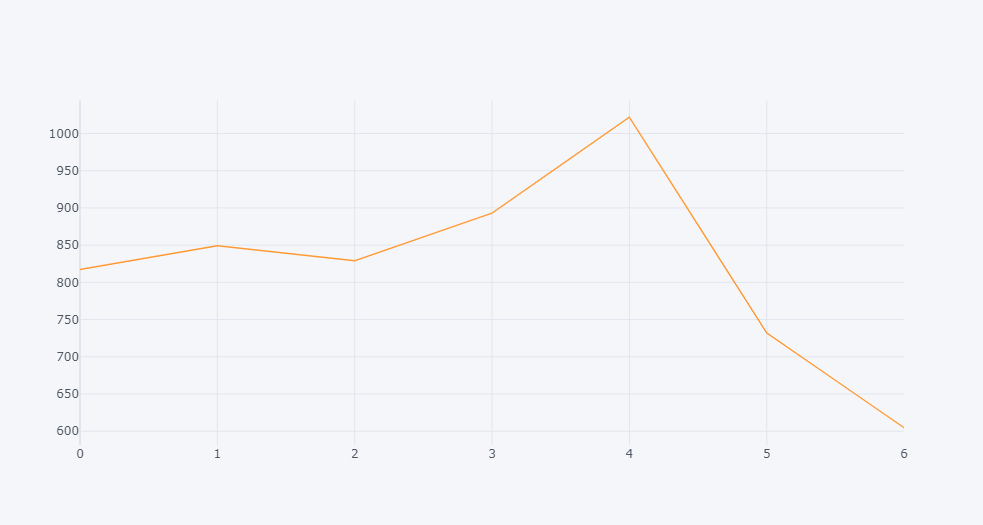
\includegraphics[width=0.5\textwidth,height=5cm]{loadondays.png}%
}
\qquad
\subfloat[]{%
  \includegraphics[width=0.5\textwidth,height=5cm]{core.png}%
}
\caption{CPU workload on day of week and CPU core Visualization }
\label{fig:core1}
\end{figure}

Figure  \ref{fig:visual} is the data visualization of hourly based data which is 2184 entries . First figure includes the  data visualizations of  performance metrics like CPU usage, Memory Usage, Network Transmitted throughput  and network received throughput. The figure  6 describe about  CPU workload  based on a days of the and CPU core used by VM in the dataset. In
Figure \ref{fig:core1}(A)  0 to 6 represent Monday to Sunday day of the week , and normally  Friday is the busiest day where most  people use VM to perform their task while Sunday is quietest day of the week.Figure \ref{fig:core1} (B)  mentioned about CPU core which used in VM to perform task, 1core CPU is widely used in this dataset while 32 core CPU is rarely used to perform big task.  
\section{Error Metrics}
For evaluating all models based on error we are using two error metrics in this project. First is RMSE (Root Mean Square Error) which uses the square root of the MSE metric. Another metric is MAE which is the Mean Absolute Error. Both equations are mentioned below.

\begin{figure}
  \centering
    
      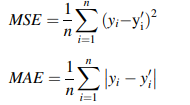
\includegraphics[width=0.3\textwidth]{errormetrics.png}
  \caption{Error metircs}
  \label{fig:error}
\end{figure}
